\chapter{Introduction}
From the rise of the smart mobile era, starting around the mid 2000s, content consumption has shifted more and more towards the mobile scene, as the mobile devices has gotten more powerful, with larger screens and Internet access has gotten more ubiquitous. Information that previously was only accessible in paper form, i.e. books and newspapers, also has had a shifting trend towards the digital platform. With all this content and information available to almost everybody and almost everywhere in the world, the importance of being able to filter it and getting only the content that is relevant or interesting to a single user is a highly relevant and an important area of research. Just as important to be able to filter this information, is how to present the filtered information. With the small screens that follows with the mobile devices, compared to for instance desktop computers, how the information is presented, is crucial to a mobile application's success.

\section{Problem}
This thesis will focus on a combination of these three main topics, namely a mobile application, with the use of a recommender system to help filter the content, narrowed down to a news application's perspective, as shown in figure \ref{thesis_focus_area}.

\begin{figure}[!htbp]
\centering
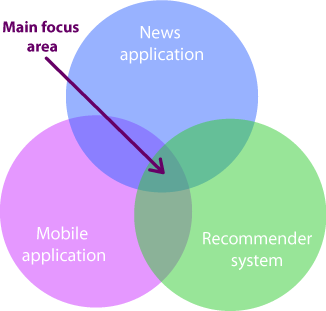
\includegraphics[width=60mm]{GFX/figures/thesisFocusArea.png}
\caption{The main focus area of the thesis.}
\label{thesis_focus_area}
\end{figure}

This will result in a mobile news recommender application, developed for iOS on the iPhone, where the main focus will be on the user interface part of the system, and how this part of the application can be created. Figure \ref{tech_news_app_architectural_view} shows how the iPhone application to be developed in association with this thesis, links to the other parts of the system as a whole. This thesis does not have as a goal to evaluate or develop recommendation and personalization techniques, but focuses on the client part of the whole news recommendation system.

\subsection{Research questions}
Following are the research questions that this thesis aims to give answers to.

\subsubsection{What are possible perspectives on news in a personalized news recommender system and how are they related?}

In which way is it possible to represent news articles and how can one view representing a news article be translated to another view. What type of information is represented in each of the different views and can one view be misleading or suffer from a lack of information compared to another view, if presented a part from the other perspectives?

Different perspectives to present news via will be presented, as well as how they are related and corresponds with each other. 


\subsubsection{What are particular features of mobile user interfaces that affect the mobile news user experience?}

In which way are mobile user interfaces different from, for instance, desktop computer user interfaces? What considerations has to be done when designing a mobile user interface and how do the interaction methods differ from one another?

The most relevant differences between a mobile user interface and other interfaces where news can be accessed will be presented. Also how these differences may have an impact on the news reading abilities on a mobile device will be discussed.


\subsubsection{What are relevant perspectives on news in current mobile news apps?}

Subjecting a handful of already developed mobile news applications, how is the news presented? Which types of perspectives are used in the different apps? Are different perspectives used in the same app, if so, how are linked together and what do they represent, in terms of information?

Approximately a dozen of commercial and non-commercial mobile news application will be targeted and the different perspectives in each application and how they are related in the application will be presented.


\subsubsection{How can these perspectives be supported on a mobile platform to increase user experience and provide maximum flexibility?}

What is the main goal for the different perspectives and are they successful in terms of presenting the information that the user wants? What do they convey and is this perspective contributing to a better user experience? Do these perspective depend on other technologies or APIs found on the mobile device, like GPS or gyroscope?

The different perspectives presented will be evaluated in terms of functionality and how they can contribute to improving the news reading experience, or on the other hand, create more confusion than supplying the user with additional useful information.


\subsubsection{The Smartmedia Mobile News Recommender Use Case}
As a use case for this thesis, the Smartmedia Mobile News Recommender system\footnote{The Smartmedia Mobile News Recommender system's project web site can be found at \url{http://smartmedia.idi.ntnu.no}.} will be applied. A mobile application will be developed on top of the existing back end, as shown in figure \ref{tech_news_app_architectural_view}, limited to the iOS platform, for the sake of simplicity.

Further the use case will be compared to existing mobile news applications in terms of available perspectives and functionality.

\section{Approach}
Following are the main approaches to answer the research questions.

\begin{enumerate}
	\item Select a particular use case to design and develop.
	\item Identify the state of commercial and non-commercial contributions, news applications and their perspectives.
	\item Compare and discuss how the contributions are related and realized.
\end{enumerate}


\section{Results}
The result of this project focuses upon identifying the state of mobile news applications that are available today, and especially how they are realized in terms of design, navigation logic, recommendation, and the mobile features to support all of this. A use case application is also a part of the result in terms of an practical approach on how to realize a mobile news recommendation application.

\section{Report Structure}

\subsubsection{Chapter \ref{chapter_theoretical_overview}: \nameref{chapter_theoretical_overview}}
A quick introduction to important terms and technologies associated with mobile devices, news applications, and recommendation.

\subsubsection{Chapter \ref{chapter_related_work}: \nameref{chapter_related_work}}
A presentation of related work done on one or more of the topics that this thesis focuses upon, mainly within some aspect of a mobile news recommender application.


\subsubsection{Chapter \ref{chapter_usecase}: \nameref{chapter_usecase}}
The presentation of the use case associated with this thesis, both front-end and back-end.


\subsubsection{Chapter \ref{chapter_perspectives}: \nameref{chapter_perspectives}}
The most common perspectives used in mobile news applications, their correlations and purpose will be presented, as well as how they are used in the different mobile news applications presented in section \ref{commercial_news_applications}.

\subsubsection{Chapter \ref{chapter_mobile_features}: \nameref{chapter_mobile_features}}
Which mobile features that are common in mobile news applications and how they are different from other systems, will be presented.

\subsubsection{Chapter \ref{chapter_comparing_applications}: \nameref{chapter_comparing_applications}}
The applications examined in section \ref{commercial_news_applications}, as well as the use case application presented in chapter \ref{chapter_usecase}, will be compared.

\subsubsection{Chapter \ref{chapter_discussion}: \nameref{chapter_discussion}}
The different perspectives' usability will be discussed, and the examined news applications will be classified into three main categories. The implementation of the use case will also be discussed.

\subsubsection{Chapter \ref{chapter_conclusion}: \nameref{chapter_conclusion}}
The conclusion drawn from this study will be presented.

\subsubsection{Chapter \ref{further_work}: \nameref{further_work}}
A set of proposals for further work will be listed and briefly explained.